\documentclass[aspectratio=169]{beamer} % 16:9 aspect ratio to match modern screens

% --- Packages ---
\usepackage[utf8]{inputenc}
\usepackage{lmodern}
\usepackage{xcolor}
\usepackage{tcolorbox}
\tcbuselibrary{skins, theorems}
\usepackage{multimedia} % Included for video support
\usepackage{fontawesome5}
\usepackage[normalem]{ulem} % The normalem option keeps your \emph{} styling normal
\usepackage{cancel}
\usepackage{amsmath}
\usepackage{tikz}
\usepackage{amssymb}
\usetikzlibrary{arrows.meta, positioning, calc}

% --- Bibliography ---
\usepackage[
	backend=bibtex,
	giveninits=true,
	style=numeric,
	maxbibnames=99,
	mincitenames=1,
	maxcitenames=4
]{biblatex}
\addbibresource{bibi.bib}
\setbeamerfont{footnote}{size=\tiny}
\setbeamercolor{footnote mark}{fg=brandAccent}

% --- Color Definitions (from theme.scss) ---
\definecolor{brandAccent}{HTML}{D77E62}
\definecolor{brandPurple}{HTML}{7201A8}
\definecolor{brandAccentDark}{HTML}{B7654B}
% Approximating the transparent #e6a08a4a background
\colorlet{brandAccentLight}{brandAccent!15!white}

\colorlet{brandRed}{brandAccent!20!red}

% --- Beamer Color & Font Settings ---
\setbeamercolor{title}{fg=brandAccent}
\setbeamercolor{frametitle}{fg=brandAccent}
\setbeamercolor{structure}{fg=brandAccent} % Colors bullets and standard structural elements
\setbeamercolor{author}{fg=black}
\setbeamercolor{date}{fg=black}

% --- Link & Reference Styling ---
\renewcommand{\eqref}[1]{\hyperref[#1]{\color{brandAccent}(\ref*{#1})}}
\hypersetup{
	colorlinks=true,
	linkcolor=brandAccent,
	urlcolor=brandAccent,
	citecolor=brandAccent
}

% Clean up the presentation (removes navigation symbols)
\setbeamertemplate{navigation symbols}{}
\setbeamertemplate{footline}[page number]

% --- Custom Theorem Block (Replicating the CSS Bubble Style) ---
\newtcbtheorem{mytheorem}{Theorem}{
	enhanced,
	colback=brandAccentLight,
	colframe=brandAccent,
	boxrule=1pt,
	arc=4mm,          % 14px border radius
	auto outer arc,
	coltitle=white,
	colbacktitle=brandAccent,
	fonttitle=\bfseries,
	% Pill-shaped floating title
	title style={borderline={0pt}{0pt}{brandAccent}, rounded corners, arc=2mm},
	attach boxed title to top left={xshift=4mm, yshift=-3mm},
	boxed title style={size=small}
}{thm}

% --- Maths ---
\def\argmin#1{{\underset{#1}{\mathrm{arg}\,\mathrm{min}\ }}}
\def\argmax#1{{\underset{#1}{\mathrm{arg}\,\mathrm{max}\ }}}

% --- Title Information ---
\title{
	\only<1>{Approximating the Score Function using Optimal Transport}
	\only<2->{\textcolor{brandRed}{\faHourglassHalf\ (Badly and Slowly)} Approximating the Score Function using Optimal Transport}
}
\subtitle{Curves and Surfaces 2026}
\author{Quentin Giton}
\institute{Laboratoire de Mathématiques d'Orsay}
\date{June 11th} % Leave empty if no date is desired

\begin{document}
	\begin{frame}
		\titlepage
	\end{frame}

	\begin{frame}[t]{Quick reminders on Optimal Transport 1/2}
		\begin{center}
			\resizebox{0.8\linewidth}{!}{
				\begin{tikzpicture}[>=Stealth, scale=1.3]
					\draw[->, thick] (-0.5, 0) -- (10.0, 0) node[right] {$\mathbb{R}$};
					
					\begin{scope}
						% Filled region for A
						\begin{scope}
							\clip (0,0) 
							.. controls (0.8, 0.1) and (1.2, 2.2) .. (2.0, 2.2)
							.. controls (2.8, 2.2) and (3.2, 0.1) .. (4.0, 0) -- (4.0,0) -- (0,0) -- cycle;
							\fill[brandAccent!30] (1.3, 0) rectangle (2.1, 2.5);
						\end{scope}
						
						\draw[thick, brandAccent] (0,0) 
						.. controls (0.8, 0.1) and (1.2, 2.2) .. (2.0, 2.2)
						.. controls (2.8, 2.2) and (3.2, 0.1) .. (4.0, 0)
						node[above=2pt] {$\mu$};
						
						\draw[brandAccent, thick, dashed] (1.3, 0) -- (1.3, 1.65);
						\draw[brandAccent, thick, dashed] (2.1, 0) -- (2.1, 2.15);
						\node[brandAccent!90!black] at (1.7, 0.8) {$\mu(A)$};
						
						\draw[brandAccent, line width=3pt] (1.3, 0) -- (2.1, 0);
						\draw[brandAccent, thick] (1.3, -0.1) -- (1.3, 0.1); 
						\draw[brandAccent, thick] (2.1, -0.1) -- (2.1, 0.1); 
						\node[brandAccent!90!black, below=4pt] at (3.125, 0) {$A=\{x\in\mathbb{R}: T(x)\in B\}$};
					\end{scope}
					
					\begin{scope}[xshift=5cm]
						% Filled region for B
						\begin{scope}
							\clip (0,0) 
							.. controls (1.0, 0.1) and (1.5, 1.4) .. (2.5, 1.4)
							.. controls (3.5, 1.4) and (3.8, 0.1) .. (4.2, 0) -- (4.2,0) -- (0,0) -- cycle;
							\fill[brandPurple!30] (1.6, 0) rectangle (3.2, 2.5);
						\end{scope}
						
						\draw[thick, brandPurple] (0,0) 
						.. controls (1.0, 0.1) and (1.5, 1.4) .. (2.5, 1.4)
						.. controls (3.5, 1.4) and (3.8, 0.1) .. (4.2, 0)
						node[above=2pt] {$\nu$};
						
						\draw[brandPurple, thick, dashed] (1.6, 0) -- (1.6, 1.025);
						\draw[brandPurple, thick, dashed] (3.2, 0) -- (3.2, 1.15);
						\node[brandPurple!90!black] at (2.4, 0.5) {$\nu(B)$};
						
						\draw[brandPurple, line width=3pt] (1.6, 0) -- (3.2, 0);
						\draw[brandPurple, thick] (1.6, -0.1) -- (1.6, 0.1); 
						\draw[brandPurple, thick] (3.2, -0.1) -- (3.2, 0.1); 
						\node[brandPurple!90!black, below=4pt] at (2.4, 0) {$B$};
					\end{scope}
					
					% DYNAMIC MAPPING ARROW
					% Slide 1: Solid Monge Arrow
					\only<1>{
						\draw[->, thick, black] (3.25, 1.5) to[bend left=30] node[above, text=black] {$T$} (6.25, 1.5);
					}
					% Slide 2: Dashed Kantorovich Arrow
					\only<2->{
						\draw[<->, thick, black, dashed] (3.25, 1.5) to[bend left=30] node[above, text=black] {$\pi$} (6.25, 1.5);
					}
				\end{tikzpicture}
			}
		\end{center}
		
		% DYNAMIC TEXT BLOCK
		\begin{itemize}
			\item Given ground cost $c(x,y)$
			
			\item 
			% Slide 1: The Monge Constraint
			\only<1>{Among all maps $T$ satisfying $\forall\textcolor{brandPurple}{B},\ \textcolor{brandPurple}{\nu(B)} = \textcolor{brandAccent}{\mu(}T^{-1}(\textcolor{brandPurple}{B})\textcolor{brandAccent}{)}$}
			% Slide 2: The Scratched Monge + The Kantorovich Constraint
			\only<2->{
				\textcolor{gray}{\sout{Among all maps $T$ satisfying $\forall B, \nu(B) = \mu(T^{-1}(B))$}} \\
				\vspace{4pt}
				Among all \textbf{transport plans} $\pi$ with marginals $\textcolor{brandAccent}{\mu}$ and $\textcolor{brandPurple}{\nu}$
			}
			
			\item 
			% Slide 1: The Monge Integral
			\only<1>{
				Find the one minimising the average transport cost
				\begin{equation*}
					\int_{\mathbb{R}^d} c(\textcolor{brandAccent}{x},T(\textcolor{brandAccent}{x}))\textcolor{brandAccent}{\mu(}\mathrm{d}\textcolor{brandAccent}{x)}
				\end{equation*}
			}
			% Slide 2: Scratched Monge Integral -> Kantorovich Integral
			\only<2->{
				\textcolor{gray}{\sout{Find the one minimising the average transport cost}}
				\begin{equation*}
					% \xcancel draws the line through the math
					\textcolor{gray}{\xcancel{\int_{\mathbb{R}^d} c(x,T(x))\mu(\mathrm{d}x)}} 
					\quad \longrightarrow \quad
					\int_{\mathbb{R}^d \times \mathbb{R}^d} c(\textcolor{brandAccent}{x},\textcolor{brandPurple}{y}) \, \pi(\mathrm{d}\textcolor{brandAccent}{x},\mathrm{d}\textcolor{brandPurple}{y})
				\end{equation*}
			}
		\end{itemize}
	\end{frame}
	
	\begin{frame}[t]{Quick reminders on Optimal Transport 2/2}
		\begin{center}
			\resizebox{0.8\linewidth}{!}{
				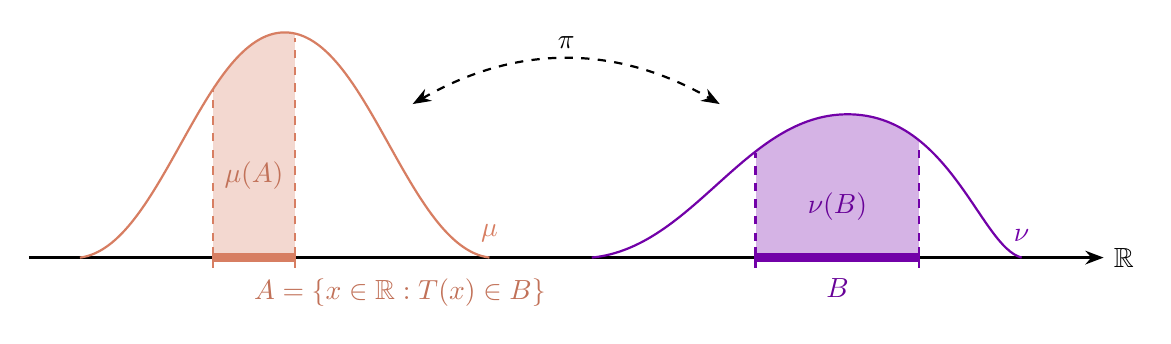
\begin{tikzpicture}[>=Stealth, scale=1.3]
					\draw[->, thick] (-0.5, 0) -- (10.0, 0) node[right] {$\mathbb{R}$};
					
					\begin{scope}
						% Filled region for A
						\begin{scope}
							\clip (0,0) 
							.. controls (0.8, 0.1) and (1.2, 2.2) .. (2.0, 2.2)
							.. controls (2.8, 2.2) and (3.2, 0.1) .. (4.0, 0) -- (4.0,0) -- (0,0) -- cycle;
							\fill[brandAccent!30] (1.3, 0) rectangle (2.1, 2.5);
						\end{scope}
						
						\draw[thick, brandAccent] (0,0) 
						.. controls (0.8, 0.1) and (1.2, 2.2) .. (2.0, 2.2)
						.. controls (2.8, 2.2) and (3.2, 0.1) .. (4.0, 0)
						node[above=2pt] {$\mu$};
						
						\draw[brandAccent, thick, dashed] (1.3, 0) -- (1.3, 1.65);
						\draw[brandAccent, thick, dashed] (2.1, 0) -- (2.1, 2.15);
						\node[brandAccent!90!black] at (1.7, 0.8) {$\mu(A)$};
						
						\draw[brandAccent, line width=3pt] (1.3, 0) -- (2.1, 0);
						\draw[brandAccent, thick] (1.3, -0.1) -- (1.3, 0.1); 
						\draw[brandAccent, thick] (2.1, -0.1) -- (2.1, 0.1); 
						\node[brandAccent!90!black, below=4pt] at (3.125, 0) {$A=\{x\in\mathbb{R}: T(x)\in B\}$};
					\end{scope}
					
					\begin{scope}[xshift=5cm]
						% Filled region for B
						\begin{scope}
							\clip (0,0) 
							.. controls (1.0, 0.1) and (1.5, 1.4) .. (2.5, 1.4)
							.. controls (3.5, 1.4) and (3.8, 0.1) .. (4.2, 0) -- (4.2,0) -- (0,0) -- cycle;
							\fill[brandPurple!30] (1.6, 0) rectangle (3.2, 2.5);
						\end{scope}
						
						\draw[thick, brandPurple] (0,0) 
						.. controls (1.0, 0.1) and (1.5, 1.4) .. (2.5, 1.4)
						.. controls (3.5, 1.4) and (3.8, 0.1) .. (4.2, 0)
						node[above=2pt] {$\nu$};
						
						\draw[brandPurple, thick, dashed] (1.6, 0) -- (1.6, 1.025);
						\draw[brandPurple, thick, dashed] (3.2, 0) -- (3.2, 1.15);
						\node[brandPurple!90!black] at (2.4, 0.5) {$\nu(B)$};
						
						\draw[brandPurple, line width=3pt] (1.6, 0) -- (3.2, 0);
						\draw[brandPurple, thick] (1.6, -0.1) -- (1.6, 0.1); 
						\draw[brandPurple, thick] (3.2, -0.1) -- (3.2, 0.1); 
						\node[brandPurple!90!black, below=4pt] at (2.4, 0) {$B$};
					\end{scope}
					
					\draw[<->, thick, black, dashed] (3.25, 1.5) to[bend left=30] node[above, text=black] {$\pi$} (6.25, 1.5);
				\end{tikzpicture}
			}
		\end{center}
		
		% DYNAMIC TEXT BLOCK
		\begin{itemize}[<+->]
			\item $p$-Wasserstein distance:
			\begin{equation*}
				W_p(\mu,\nu)^p = \inf_{\pi\in\Pi(\mu,\nu)} \int d(x,y)^p \gamma(\mathrm{d}x,\mathrm{d}y)
			\end{equation*}
			\item Kantorovich duality
			\begin{equation*}
				\inf_{\pi\in\Pi(\mu,\nu)} \int c(x,y) \gamma(\mathrm{d}x,\mathrm{d}y) = \sup_{\phi} \int \phi(x)\mu(\mathrm{d}x)+\int\phi^c(y)\nu(\mathrm{d}y),
			\end{equation*}
			where $\phi^c(y) := \inf_x c(x,y)-\phi(x)$.
		\end{itemize}
	\end{frame}
	
	\begin{frame}{What is the score function?}
		\begin{itemize}[<+->]
			\item \textbf{Forward Process (Heat Dissipation):} 
			Running the SDE forward diffuses our data into pure noise. The density follows a Fokker-Planck equation (akin to the heat equation):
			\begin{equation*}
				\mathrm{d}x_t = f(x_t, t) \, \mathrm{d}t + g(t) \, \mathrm{d}w_t
			\end{equation*}
			
			\item \textbf{Reverse Process (Reversing Entropy):} 
			To reverse this natural dissipation, we must inject a highly specific, restoring drift back into the system:
			\begin{equation*}
				\mathrm{d}x_t = \Big[ f(x_t, t) - g(t)^2 \underbrace{\textcolor{brandRed}{\nabla \log p_t(x_t)}}_{\text{\textbf{The Score Function}}} \Big] \mathrm{d}t + g(t) \, \mathrm{d}\bar{w}_t
			\end{equation*}
			
			\item \textbf{The Physical Intuition:}
			\begin{itemize}
				\item We can view the system through a potential energy landscape: $E_t(x) = -\log p_t(x)$.
				\item The score is simply the negative gradient of this energy: $\textcolor{brandRed}{\nabla \log p_t(x)} = -\nabla E_t(x)$.
				\item \textbf{Conclusion:} The score acts as the exact thermodynamic \textbf{force} required to fight the heat equation and push the dispersed particles back into their highly-structured original states.
			\end{itemize}
		\end{itemize}
	\end{frame}
	
	
	
	\begin{frame}{Using OT to learn the score}
		Consider $v_t = -\nabla(\ln{\rho_t}+V)$ where $V(x)=\frac{\|x\|^2}{2}$. Then, the Fokker-Planck equation
		\begin{equation*}
			\partial_t\rho_t = \Delta\rho_t + \mathrm{div}(\rho_t\nabla V).
		\end{equation*}
		\pause
		\begin{itemize}
			\item transports any initial condition $\rho_0\in\mathcal{P}(\mathbb{R^d})$ towards the standard Gaussian $\gamma=\mathcal{N}(0,Id)$ and
			\item can be seen as the Wasserstein gradient flow of the energy \footfullcite{jordan_variational_1998}
			\begin{equation*}
				\mathcal{F}(\rho):=\int V\rho+\int\rho\ln{\rho}
			\end{equation*}
		\end{itemize}
	\end{frame}
	
	
	
	\begin{frame}{Using OT to learn the score}
		We can discretize in time the gradient flow using implicit Euler scheme (or \textbf{JKO scheme}):
		\begin{equation}\label{eq:JKO}
			\rho_{n+1}^\tau := \argmin{\rho\in\mathcal{P}_2(\mathbb{R}^d)} \left\{ \mathcal{F}(\rho)+\frac{1}{2\tau}W_2(\rho,\rho_n^\tau)^2 \right\}
		\end{equation}
		\pause
		As explained by Santambrogio in his book \footfullcite{santambrogio_optimal_2015}, we have
		\begin{equation*}
			\nabla\psi_n^{c_\tau} = v_{n\tau} = -\nabla(\ln{\rho_{n+1}^\tau}+V),
		\end{equation*}
		where $\psi_n^{c_\tau}$ is a Kantorovich potential related to the transport from $\rho_n^\tau$ to $\rho_{n+1}^\tau$. Therefore approximating the score amounts to approximating $\nabla\psi_n^{c_\tau}$.
	\end{frame}
	
	
	
	
	
	
	
	
	
	
	
	
	
	
	
	
	
	
	
	
	
	
	
	
	
	
	
	
	
	
	
	
	% --- Theorem Slide (Replicating Slide 9) ---
	\begin{frame}{Stochastic Gradient Descent}
		\begin{mytheorem}{}{}
			If $\alpha_k=\frac{R}{B\sqrt{k}}$, then
			\[
			\forall T\geq 1,\quad \mathbb{E}\left[ G_{n}^{\tau}(\bar{\theta}_{T}^n)-G_{n}^{\tau}(\theta^{\tau}_{n}) \right]\leq BR\left(\frac{2}{T}+\frac{1}{\sqrt{T}}\right),
			\]
		\end{mytheorem}
		\vspace{1em}
		where $\bar{\theta}_{T}^n$ denotes the arithmetic mean of the family $(\theta^{(k)})_{k=1}^{T}$ and $B$ depends only on $R$ and $\sup_x \|\phi(x)\|$.
	\end{frame}
	
	% --- Video Implementation Example ---
	\begin{frame}{Some animations}
		\begin{center}
			% Usage: \movie[options]{poster text or image}{video_file.mp4}
			% Note: You need a compatible PDF viewer (like pdfpc or Okular) to play this.
			\movie[width=0.6\textwidth, height=0.4\textwidth, poster, showcontrols]
			{\color{brandAccent} Click here to play video}{medias/forward.mp4}
		\end{center}
	\end{frame}
	
	% --- Final Slide (Centered) ---
	\begin{frame}[c]
		\begin{center}
			\usebeamercolor[fg]{title}\Large\bfseries Thank you for your attention!
		\end{center}
	\end{frame}
	
\end{document}